\chapter[Metodologia Científica]{Metodologia Científica}
\addcontentsline{toc}{chapter}{Metodologia Científica}
\markboth{Metodologia Científica}{Metodologia Científica}

Este capítulo apresenta a metodologia utilizada para o desenvolvimento deste projeto, fundamentando os processos adotados na criação do jogo eletrônico inspirado em *Tron: Light Cycles*. A proposta do trabalho é orientar o desenvolvimento com base em abordagens bem estabelecidas, como o Scrum e o MDA (Mecânica, Dinâmica e Estética), garantindo que cada etapa seja sistematizada e documentada de forma clara.

Além disso, são detalhadas as estratégias de modelagem aplicadas ao projeto, bem como as ferramentas utilizadas, como Godot, GDScript e Aseprite, que permitiram o desenvolvimento e a implementação do jogo. Essas escolhas têm como objetivo não apenas a entrega de um produto funcional, mas também a criação de uma base didática para futuros desenvolvedores.

\section{Scrum}

O Scrum é uma metodologia ágil que foi escolhida para gerenciar o desenvolvimento do projeto devido à sua capacidade de promover colaboração, flexibilidade e iterações rápidas. Essa abordagem divide o projeto em ciclos curtos, chamados \textit{sprints}, que têm duração definida e objetivos claros. Ao final de cada sprint, é possível revisar os resultados alcançados e ajustar o planejamento para os próximos passos \cite{schwaber2013}.

No contexto deste projeto, o Scrum foi adaptado para permitir o desenvolvimento iterativo do jogo. Cada sprint envolveu as seguintes etapas:

\begin{itemize}
  \item \textbf{Planejamento:} Definição das tarefas prioritárias, como implementação de mecânicas, design de níveis e testes.
  \item \textbf{Execução:} Desenvolvimento das funcionalidades planejadas, utilizando as ferramentas escolhidas.
  \item \textbf{Revisão:} Testes e validação das funcionalidades implementadas, com foco na experiência do usuário.
\end{itemize}

Mesmo em um projeto individual, o uso do Scrum promove organização das etapas e entrega contínua de resultados tangíveis. Para montar o cronograma, foi considerado o período de 2 meses e meio para elaboração do trabalho, com sprints de duas semanas.

\begin{table}[H]
\centering
\caption{Requisitos funcionais do jogo}
\label{tab:requisitos}
\begin{tabular}{|c|p{3cm}|p{7.5cm}|c|}
\hline
\textbf{ID} & \textbf{Requisito} & \textbf{Descrição} & \textbf{Prioridade} \\ \hline
RF01 & Criar e gerenciar salas de jogo & Permitir que até 6 jogadores ingressem e joguem juntos em uma mesma sala. & Alta \\ \hline
RF02 & Controlar os personagens & O jogador deve conseguir movimentar seu personagem para esquerda ou direita. & Alta \\ \hline
RF03 & Gerar e exibir o rastro & Cada jogador deixa um rastro letal no mapa, exceto nos pontos de brechas aleatórias. & Alta \\ \hline
RF04 & Aplicar regras de pontuação & O jogo deve calcular a pontuação conforme a fórmula definida e exibir o placar. & Média \\ \hline
RF05 & Implementar poderes especiais & Os poderes devem surgir aleatoriamente no mapa e ser ativados pelo jogador que os coletar. & Alta \\ \hline
RF06 & Detectar colisões & O jogo deve encerrar a rodada quando um jogador colidir com um rastro ou com a parede. & Alta \\ \hline
RF07 & Reposicionar os jogadores & Após cada rodada, os jogadores devem ser reposicionados nas posições iniciais. & Média \\ \hline
RF08 & Exibir feedback visual e sonoro & O jogo deve apresentar efeitos visuais e sonoros ao ativar poderes, colidir ou vencer a partida. & Média \\ \hline
\end{tabular}

\vspace{0.3em}
\small \textbf{Fonte:} Elaboração própria.
\end{table}

\begin{table}[H]
\centering
\caption{Requisitos não funcionais}
\label{tab:requisitos-nao-funcionais}
\begin{tabular}{|c|p{4cm}|p{6cm}|c|}
\hline
\textbf{ID} & \textbf{Requisito} & \textbf{Descrição} & \textbf{Prioridade} \\
\hline
RNF01 & Engine de desenvolvimento & O jogo deve ser desenvolvido na Godot Engine devido à sua leveza e suporte a 2D. & Alta \\
\hline
RNF02 & Suporte multiplataforma & O jogo deve ser compatível com Windows e Linux. & Média \\
\hline
RNF03 & Desempenho otimizado & O jogo deve rodar a pelo menos 60 FPS em hardware modesto. & Média \\
\hline
RNF04 & Interface responsiva & O jogo deve apresentar uma interface clara e intuitiva para facilitar o entendimento das mecânicas. & Alta \\
\hline
RNF05 & Código modular e expansível & O código deve ser estruturado de forma a permitir futuras adições e melhorias sem grandes refatorações. & Alta \\
\hline
RNF06 & Conectividade com controle Xbox & O usuário pode conectar um controle analógico e o game deve poder reconhecer o dispositivo. & Baixa \\
\hline
RNF07 & Tratamento de bugs & Os bugs do jogo não devem atrapalhar a jogabilidade. & Alta \\
\hline
\end{tabular}

\vspace{0.3em}
\small \textbf{Fonte:} Elaboração própria.
\end{table}


\begin{table}[H]
\centering
\caption{Cronograma de desenvolvimento}
\label{tab:cronograma}
\begin{tabular}{|p{4cm}|p{2.5cm}|p{5.5cm}|p{3cm}|}
\hline
\textbf{Sprint} & \textbf{Duração} & \textbf{Objetivo} & \textbf{Requisitos envolvidos} \\
\hline
Sprint 1 - Planejamento e Configuração & 2 semanas & Configurar ambiente na Godot, estruturar projeto, definir assets básicos e movimentação inicial. & RF01, RF02, RNF01, RNF02 \\
\hline
Sprint 2 - Mecânicas Básicas & 2 semanas & Implementar colisões, rastros de luz e regras fundamentais da partida. & RF03, RF05 \\
\hline
Sprint 3 - Implementação dos Poderes & 2 semanas & Criar e integrar poderes especiais, garantindo variedade e equilíbrio. & RF06 \\
\hline
Sprint 4 - Interface e Experiência do Usuário & 2 semanas & Criar menus, HUD, sistema de pontuação e feedback visual para melhor UX. & RNF04, RF04 \\
\hline
Sprint 5 - Testes e Ajustes de Jogabilidade & 2 semanas & Testar fluxo do jogo localmente, ajustar balanceamento e melhorar usabilidade. & RF08, RNF03, RNF05, RF07 \\
\hline
Sprint 6 - Refinamento e correção de bugs & 1 semana & Revisão final, correção de bugs e otimizações. & RNF07, RNF06 \\
\hline
\end{tabular}

\vspace{0.3em}
\small \textbf{Fonte:} Elaboração própria.

\end{table}

A metodologia Scrum foi escolhida por já fazer parte do repertório de práticas com as quais havia familiaridade. Ter experiência prévia facilita a aplicação e torna mais simples adaptar a técnica ao contexto de um projeto individual. Como não se trata de um trabalho em equipe, nem todos os ritos tradicionais foram seguidos. Optou-se por aplicar apenas o que realmente faria diferença na organização e ritmo de trabalho. No desenvolvimento espera-se observar como essas técnicas foram utilizadas.


\section{MDA (Mecânica, Dinâmica e Estética)}

O modelo MDA foi adotado como base para estruturar os elementos do jogo. Este modelo é amplamente utilizado no desenvolvimento de jogos digitais por oferecer uma perspectiva clara sobre como cada componente de um jogo contribui para a experiência do jogador. Assim como o autor Johan Huizinga, o estudo feito por Hunicke em \textit{“MDA: A Formal Approach to Game Design and Game Research”} formaliza o consumo dos jogos em três componentes distintos e estabelece uma relação de contraparte para o desenvolvimento de jogos \cite{hunicke2004}:

\begin{figure}[htbp]
    \centering
    \caption{Componentes de um jogo modelo MDA}
    \label{fig:mda-comp}
    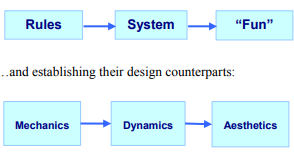
\includegraphics[width=0.7\textwidth]{figuras/hunicke.png}
    \legend{Fonte: HUNICKE, Robin; LEBLANC, Marc; ZUBEK, Robert. MDA: A Formal Approach to Game Design and Game Research. 2004. p. 2.}
\end{figure}

Para entender melhor o que é cada camada, fazemos a seguinte descrição:

\begin{itemize}
    \item \textbf{Mecânica}: Refere-se às regras, interações e sistemas que governam o funcionamento do jogo. No contexto do \textit{Light Cycles}, inclui aspectos como o controle do veículo, a criação de barreiras luminosas e a detecção de colisões.
    
    \item \textbf{Dinâmica}: Diz respeito às interações emergentes resultantes da aplicação das mecânicas. Exemplos incluem o comportamento dos jogadores ao tentar ``trancar'' os oponentes ou escapar de barreiras.
    
    \item \textbf{Estética}: Envolve a experiência emocional e sensorial do jogador. Neste projeto, busca-se criar uma experiência visual simples, uma vez que o tempo é curto e o foco está no conteúdo funcional e didático.
\end{itemize}

O uso do MDA possibilita uma abordagem holística no desenvolvimento do jogo, alinhando os aspectos técnicos à experiência pretendida para os jogadores \cite{carroll2000}.

Com base nessas definições, foram elaboradas as respectivas tabelas de Mecânica, Dinâmica e Estética do jogo proposto.

\begin{table}[H]
\centering
\caption{MDA: Mecânicas do jogo}
\label{tab:mecanicas}
\begin{tabularx}{\textwidth}{|l|X|X|}
\hline
\textbf{Mecânicas} & \textbf{Descrição} & \textbf{Observação} \\
\hline
Movimentação & O jogador pode girar para a esquerda ou para a direita, sendo a curva maior conforme a velocidade. & A mecânica exige precisão e estratégia para evitar colisões. \\
\hline
Rastros & Cada jogador deixa um rastro letal ao se movimentar, criando barreiras no cenário. & Brechas aleatórias surgem ocasionalmente nos rastros, permitindo a passagem. \\
\hline
Poderes Especiais & Jogadores podem coletar poderes aleatórios que afetam a jogabilidade. & Alguns poderes afetam apenas o jogador, enquanto outros impactam todos. \\
\hline
Colisão e eliminação & O jogador que colidir com uma parede ou rastro é eliminado da rodada. & A rodada continua até restar apenas um jogador vivo. \\
\hline
Sistema de pontos & A cada rodada, jogadores recebem pontos conforme sua colocação. & O jogo termina quando um jogador atinge a pontuação necessária. \\
\hline
\end{tabularx}

\vspace{0.3em}
\small \textbf{Fonte:} Elaboração própria.
\end{table}


\begin{table}[H]
\centering
\caption{MDA: Estética e Dinâmicas}
\label{tab:mda-estetica-dinamica}
\begin{tabularx}{\textwidth}{|>{\raggedright\arraybackslash}X|>{\raggedright\arraybackslash}X|}
\hline
\textbf{Estética} & \textbf{Dinâmicas} \\
\hline
Competição & Os jogadores disputam a sobrevivência, tentando eliminar os oponentes. \\
\hline
Desafio & A necessidade de reflexos rápidos e pensamento estratégico cria uma experiência intensa. \\
\hline
Estratégia & O uso inteligente dos rastros e poderes pode definir a vitória. \\
\hline
Satisfação & Jogadas bem executadas e vitórias são gratificantes para o jogador. \\
\hline
Caos e imprevisibilidade & Os poderes aleatórios e as brechas nos rastros tornam cada rodada única. \\
\hline
Surpresa & Momentos inesperados ocorrem constantemente, mantendo o jogo dinâmico. \\
\hline
Pressão crescente & Conforme a partida avança, o espaço no mapa fica mais restrito, aumentando a tensão. \\
\hline
Imersão & O ritmo acelerado e a disputa constante mantêm os jogadores envolvidos. \\
\hline
\end{tabularx}

\smallskip
\small \textbf{Fonte:} Elaboração própria.
\end{table}

\subsection{Estratégias de Modelagem}

Para garantir a consistência e qualidade do projeto, foram empregadas estratégias de modelagem baseadas em princípios da Engenharia de Software. As etapas adotadas no processo de desenvolvimento do jogo visam estruturar o fluxo de trabalho de maneira eficiente e \textit{iterativa}, permitindo não apenas a construção do jogo, mas também a criação de um conteúdo funcional e didático para futuras implementações e para o aprendizado de novos desenvolvedores \cite{sommerville2011}.

\begin{flushright}
\begin{minipage}{0.85\textwidth}
\begin{quote}
``[...]\textit{Os modelos são usados durante o processo de engenharia de requisitos para ajudar a extrair os requisitos do sistema; durante o processo de projeto, são usados para descrever o sistema para os engenheiros que o implementam; e, após isso, são usados para documentar a estrutura e a operação do sistema.}''

\cite{sommerville2011}, p. 82.
\end{quote}
\end{minipage}
\end{flushright}

As seguintes estratégias foram usadas:

\begin{itemize}
    \item \textbf{Levantamento de Requisitos:} A primeira etapa foi a identificação das funcionalidades essenciais do jogo. Isso incluiu a definição dos controles responsivos, garantindo que os jogadores tivessem uma experiência fluida e intuitiva, a criação de uma interface gráfica simples e acessível, e o balanceamento das mecânicas do jogo. O levantamento de requisitos foi fundamental para alinhar as expectativas do produto com as necessidades dos jogadores, além de facilitar as decisões durante o processo de desenvolvimento.

    \item \textbf{Modelagem de Dados:} Após o levantamento de requisitos, foi realizada a modelagem de dados, que envolveu a estruturação de informações sobre os cenários do jogo, personagens, eventos e interações. O objetivo foi organizar os dados de forma que a implementação das funcionalidades fosse eficiente, sem redundâncias e com alto desempenho. A modelagem de dados também serviu como base para a criação de scripts e animações dentro da engine utilizada, o que contribuiu para a integração das mecânicas de forma coesa.

    \item \textbf{Prototipagem:} A prototipagem foi uma etapa relevante para validar as mecânicas do jogo antes de sua implementação final. Modelos iniciais das interações e funcionalidades foram criados, permitindo testar as ideias em um estágio inicial e fazer ajustes rápidos com base no feedback obtido. A prototipagem não só acelerou o processo de desenvolvimento, mas também proporcionou uma visão prática de como as mecânicas poderiam ser experienciadas pelos jogadores, ajudando na identificação de melhorias e possíveis problemas de usabilidade.
\end{itemize}

A adoção dessas estratégias de modelagem visa proporcionar um processo de desenvolvimento mais organizado e focado, com potencial para resultar em um produto funcional e didático, que possa contribuir para a aprendizagem de desenvolvedores iniciantes.

\subsubsection{Modelo de Caso de Uso}

A modelagem de casos de uso, conforme definido por Sommerville (2011), é uma técnica essencial na engenharia de software para elicitar e especificar os requisitos funcionais de um sistema. Um caso de uso representa uma interação entre um ator (um usuário ou outro sistema) e o sistema em si, descrevendo uma sequência de ações que o ator realiza para atingir um objetivo específico.

No contexto do desenvolvimento de jogos, a modelagem de casos de uso oferece uma maneira clara e concisa de descrever as interações dos jogadores com o jogo, auxiliando no projeto e implementação das funcionalidades. A abordagem escolhida para o jogo da cobrinha 2D buscou representar as ações dos jogadores e as mecânicas do jogo de forma abrangente, utilizando um diagrama de casos de uso que incorpora elementos como atores, casos de uso, relacionamentos (\textit{include} e \textit{extend}) e anotações.

\textbf{Atores}
Os atores, Jogador 1 e Jogador 2, representam os jogadores humanos que interagem com o jogo. Eles são os iniciadores das ações e se beneficiam das funcionalidades oferecidas pelo jogo.

\textbf{Casos de Uso}
Os casos de uso descrevem as ações que os jogadores podem realizar ou que ocorrem como parte do jogo:

\begin{itemize}
  \item \textbf{Jogar}: Abrange toda a experiência do jogador no jogo, desde o início até o fim.
  \item \textbf{Mover}: Representa a ação do jogador de controlar a direção da cobrinha (esquerda ou direita).
  \item \textbf{Coletar Poder}: Descreve a mecânica do jogo em que a cobrinha coleta automaticamente um poder ao passar por cima do item.
  \item \textbf{Colidir}: Representa o evento em que a cobrinha colide com a parede ou com o próprio corpo.
  \item \textbf{Morrer}: Descreve o resultado da colisão, em que a cobrinha perde uma vida ou o jogo termina.
  \item \textbf{Mudar Direção}: Ação do jogador de controlar a cobrinha para a esquerda ou para a direita.
  \item \textbf{Poder Vermelho/Verde/Azul}: Representam os diferentes tipos de poderes que a cobrinha pode coletar, cada um com efeitos específicos.
  \item \textbf{Rodada}: Descreve o ciclo de jogo, desde o início até o fim, com um número definido de rodadas.
  \item \textbf{Fim da rodada}: Representa o momento em que uma rodada termina, seja por um jogador perder ou por outros critérios.
  \item \textbf{Ganhar pontos}: Ação de receber pontos ao final de uma rodada, de acordo com o desempenho.
  \item \textbf{Jogo}: Representa a partida completa, com várias rodadas e o objetivo de atingir um limite de pontos.
  \item \textbf{Fim do Jogo}: Ocorre quando um jogador atinge o limite de pontos ou quando todas as rodadas são concluídas.
  \item \textbf{Limite de Pontos}: Condição para o fim do jogo, em que um jogador precisa atingir uma pontuação específica.
\end{itemize}

\textbf{Relacionamentos}

\textbf{Include}: O relacionamento \textit{include} (\textless\textless include\textgreater\textgreater) é utilizado para indicar que um caso de uso é parte integrante de outro. Por exemplo, ``Jogo'' inclui ``Rodada'', ``Rodada'' inclui ``Fim da Rodada'' e ``Fim da Rodada'' inclui ``Ganha Pontos''.

\textbf{Extend}: O relacionamento \textit{extend} (\textless\textless extend\textgreater\textgreater) é utilizado para representar variações ou extensões de um caso de uso. Por exemplo, ``Mover'' pode ser estendido por ``Colidir'' e ``Mudar Direção'' pode ser estendido por ``Coletar Poder''.

\begin{figure}[htbp]
    \centering
    \caption{Diagrama casos de uso}
    \label{fig:use-case}
    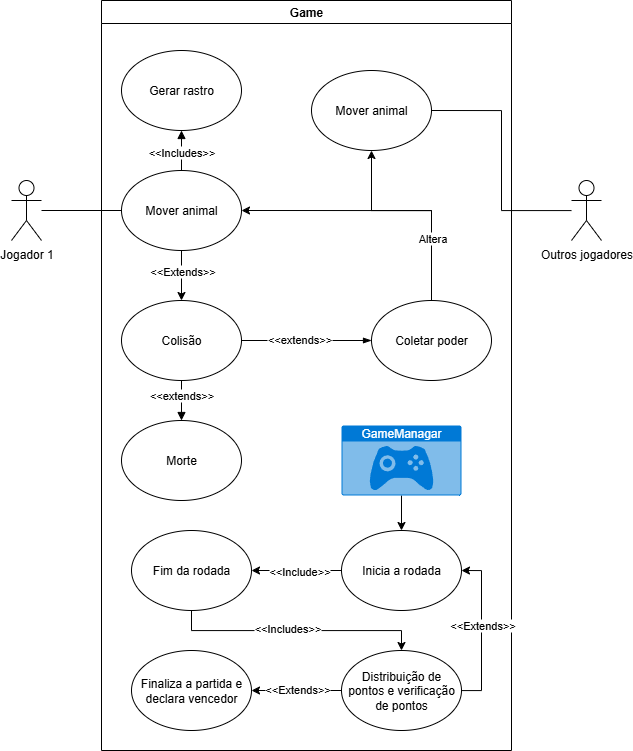
\includegraphics[width=0.7\textwidth]{figuras/diagrama-uso.png}
    \legend{Fonte: Elaboração própria.}
\end{figure}